\documentclass{jsarticle}
\usepackage[margin = .7in]{geometry}
\usepackage[dvipdfmx]{graphicx}
\usepackage{listings}
\usepackage{amsmath}
\usepackage{amsfonts}
\usepackage{bm}
\lstset{%
  language={python},
  basicstyle={\small},%
  identifierstyle={\small},%
  commentstyle={\small\itshape},%
  keywordstyle={\small\bfseries},%
  ndkeywordstyle={\small},%
  stringstyle={\small\ttfamily},
  frame={tb},
  breaklines=true,
  columns=[l]{fullflexible},%
  numbers=left,%
  xrightmargin=0zw,%
  xleftmargin=3zw,%
  numberstyle={\scriptsize},%
  stepnumber=1,
  numbersep=1zw,%
  lineskip=-0.5ex%
}

\begin{document}
\title{卒論テーマ候補 :満員電車}
\author{池上 慧}
\maketitle

\section{目的}
満員電車の緩和を目指す。このモデルでは各人が限定的であれprivate informationを申告することで社会的な損失を軽減できるかを考える。最終的には、正直申告をさせるメカニズムに基づいて実際に乗車時間を事前に投票するアプリを用い、情報の事前開示が乗車行動に望ましい変化をもたらしたかを検証する実証研究につなげたい。

\section{モデルの分析}
電車の候補が全部で$M$本とし、$j \in M$で各電車を指すとする。プレイヤーは$N$人で$i$をインデックスとする。プレイヤー$i$が電車$j$に乗車することの効用$(V_j^i)$は、その電車の発車時刻$(t_j)$に紐付いた$i$ごとに異なる価値$(u_j^i)$と、その電車に乗車するプレイヤーの数$(N_j)$に依存して決定する。ただし$\left\{u_j^i\right\}$は自身の持つ各電車への価値は自分で認識できるが、自分以外のプレイヤーが持つ各電車への価値は認識できないとする。ここでそれぞれの効用への寄与は分離できるとして、
\begin{align*}
	V_j^i = u_j^i + g(N_j)
\end{align*}
で書くことができるとする。

しかし、実際に乗車する電車を決定する際には、実現する乗車人数$N_j$に基づいて意思決定することはできない。なぜならまだその人数は実現していないからである。そのため、$N_j$についての期待値に基づいて意思決定を下すことになる。ここで、プレイヤー同士にも、経済学者にも観測できない撹乱項$\epsilon_j^i$が電車とプレイヤーについて独立に第1種極値分布にしたがうと仮定し、$additive$に効用に影響するとする。すなわち、
\begin{align*}
	h_j^i = V_j^i + \epsilon_j^i = u_j^i + g(N_j) + \epsilon_j^i
\end{align*}
でプレイヤー$i$の持つ電車$j$の効用をかけるとし、$N_j$について期待値をとった形で
\begin{align*}
	{h_j^i}^* = {V_j^i}^* + \epsilon_j^i = u_j^i + E[g(N_j)] + \epsilon_j^i
\end{align*}
と書くとする。
この時、$g(N_k) = \alpha N_k$として特定化すると、プレイヤー$i$が電車$j$を選ぶ確率は以下のようにかける。
\begin{align*}
	p_j^i = Pr(\text{i chooses j}) = P({h_j^i}^* \geq {h_{j^{'}}^i}^*\ \text{for all}\ j \in M) = \frac{\exp({V_j^i}^*)}{\sum_k \exp({V_k^i}^*)} = \frac{\exp(u_j^i + \alpha E[N_j])}{\sum_k \exp(u_k^i + \alpha E[N_k])}
\end{align*}

以下、簡単のためにプレイヤーの数と電車の数を共に$2$としてモデルを分析する。$p_2^1 = 1 - p_1^1$と$p_2^2 = 1 - p_1^2$より、先の結果を書き下すと、
\begin{align*}
	\begin{cases}p_1^1 &= \frac{1}{1 + \exp(u_2^1 - u_1^1 + 2\alpha(1 - p_1^1 - p_1^2))} \\[10pt]
	p_1^2 &= \frac{1}{1 + \exp(u_2^2 - u_1^2 + s\alpha(1 -p_1^1 -p_1^2))}
	\end{cases}
\end{align*}
のようにかける。

解釈として、$\left\{ p_j^i\right\}$は確率そのものではなく、新たに得られた各電車への効用であると見ることとする。すなわち、$p_j^i > p_{j^{'}}^i$の時、プレイヤー$i$は電車$j$を電車$j^{'}$よりも選好していると解釈し、またその時実際に電車$j$を選ぶという行動をとるとする。この時、「プレイヤー$1$が電車$1,2$について無差別である」という事象は、$p_2^1 = p_1^1 \Leftrightarrow p_2^1 = p_1^1 = \frac{1}{2}$であるということを指す。

$\alpha \neq 0$と仮定すると、
\begin{align*}
	&\frac{1}{2} = p_1^1\\[8pt]
	\Leftrightarrow\quad&\frac{1}{2} = \frac{1}{1 + \exp(u_2^1 - u_1^1 + 2\alpha(1 - p_1^1 - p_1^2))}\\[8pt]
	\Leftrightarrow\quad &u_2^1 - u_1^1 + 2\alpha(1 - p_1^1 - p_1^2)) = 0\\[8pt]
	\Leftrightarrow\quad &p_1^2 = \frac{u_2^1 - u_1^1}{2\alpha} + \frac{1}{2}\\[8pt]
	\Leftrightarrow\quad &\frac{1}{1 + \exp(u_2^2 - u_1^2 + s\alpha(1 -p_1^1 -p_1^2))} = \frac{u_2^1 - u_1^1 + \alpha}{2\alpha}\\[8pt]
	\Leftrightarrow\quad &\alpha - (u_2^1 - u_1^1) = (\alpha + u_2^1 - u_1^1)\exp(u_2^2 - u_1^2 + 2\alpha(1 - p_1^1 - p_1^2))\\[8pt]
	\Leftrightarrow\quad &\alpha - (u_2^1 - u_1^1) = (\alpha + u_2^1 - u_1^1)\exp(u_2^2 - u_1^2 - (u_2^1 - u_1^1))\\[8pt]
	\Leftrightarrow\quad &\exp(u_2^2 - u_1^2 - (u_2^1 - u_1^1)) = \frac{\alpha - (u_2^1 - u_1^1)}{\alpha + (u_2^1 - u_1^1)}\\[8pt]
	\Leftrightarrow\quad &(u_2^2 - u_1^2) - (u_2^1 - u_1^1) = {\rm log}\ (\alpha - (u_2^1 - u_1^1)) - {\rm log}\ (\alpha + (u_2^1 - u_1^1))
\end{align*}
ここで右辺の各項をマクローリン展開する。
\begin{align*}
	&{\rm log}\ (\alpha + x) \approx {\rm log}\ \alpha + \frac{1}{\alpha} x\\
	&{\rm log}\ (\alpha - x) \approx {\rm log}\ \alpha - \frac{1}{\alpha} x
\end{align*}
なので、
\begin{align*}
	&{\rm log}\ (\alpha + (u_2^1 - u_1^1)) \approx {\rm log}\ \alpha + \frac{1}{\alpha} (u_2^1 - u_1^1)\\
	&{\rm log}\ (\alpha - (u_2^1 - u_1^1)) \approx {\rm log}\ \alpha - \frac{1}{\alpha} (u_2^1 - u_1^1)
\end{align*}
であり、先の式は以下で近似できる。ただし$d_i = u_2^i - u_1^i$としている。
\begin{align*}
	&(u_2^2 - u_1^2) - (u_2^1 - u_1^1) = -\frac{2}{\alpha} (u_2^1 - u_1^1)\\
	\Leftrightarrow\quad &(u_2^2 - u_1^2) = (1-\frac{2}{\alpha})(u_2^1 - u_1^1)\\
	\Leftrightarrow\quad &d_2 = (1-\frac{2}{\alpha})d_1
\end{align*}
以上より、自分以外のタイプ、ここでは$\left\{ d_i\right\}$を知っている時のプレイヤー1の最適反応は以下のようである。
\begin{align*}
	\begin{cases}&\text{1 chooses 1} \quad \text{if}\ d_2 > (1 - \frac{2}{\alpha})d_1\\[8pt]
	&\text{indifferent} \quad \text{if}\ d_2 = (1 - \frac{2}{\alpha})d_1\\[8pt]
	&\text{1 chooses 2} \quad \text{if}\ d_2 < (1 - \frac{2}{\alpha})d_1
	\end{cases}
\end{align*}
プレイヤー2についても同様の最適反応関数が以下のように書ける。
\begin{align*}
	\begin{cases}&\text{2 chooses 1} \quad \text{if}\ d_1> (1 - \frac{2}{\alpha})d_2\\[8pt]
	&\text{indifferent} \quad \text{if}\ d_1 = (1 - \frac{2}{\alpha})d_2\\[8pt]
	&\text{2 chooses 2} \quad \text{if}\ d_1 < (1 - \frac{2}{\alpha})d_2
	\end{cases}
\end{align*}
以上の最適反応を$(d_1, d_2)$平面上で考えると、$\alpha < 0$の仮定の下で図示できる。
\begin{figure}[h]
    \centering
    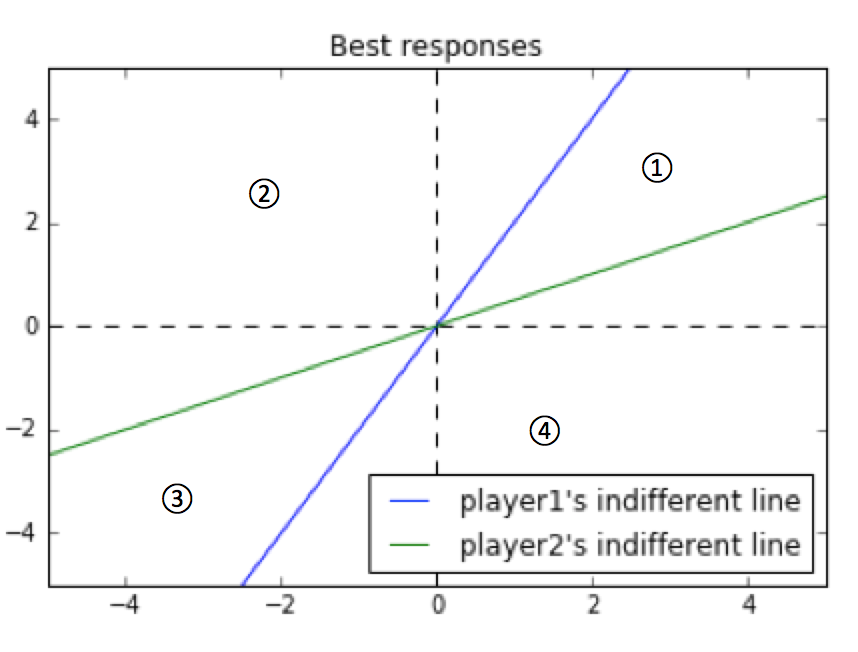
\includegraphics[width=10cm]{BR.png}
    \caption{indifferent curves when $\alpha = -2$}
\end{figure}
$[a, b]$でプレイヤー$1$が電車$a$を、プレイヤー$2$が電車$b$を選ぶことを表現する。これを用いて、相手のタイプが完全にわかっている場合に合理的な行動の結果とられる戦略の組は以下のようであることがわかる。
\begin{align*}
	\begin{cases}
		&[2, 2]\ \text{if}\ (d_1, d_2) \in \text{area 1}\\[8pt]
		&[1, 2]\ \text{if}\ (d_1, d_2) \in \text{area 2}\\[8pt]
		&[1, 1]\ \text{if}\ (d_1, d_2) \in \text{area 3}\\[8pt]
		&[2, 1]\ \text{if}\ (d_1, d_2) \in \text{area 4}\\[8pt]
	\end{cases}
\end{align*}

今簡単のために$d_i \sim N(0,1)\ \forall\ i$とする(global gameのように自分の情報から相手の分布をベイズ推論する方が面白いかも)。プレイヤー$i$は$d_i$のみを観測しているので$d_2$の情報も必要な、上の領域に従った行動の決定はできない。しかしここで$d_i \sim N(0,1)\ \forall\ i$を知っているとすると、自身のタイプである$d_i$に従って、各電車についての最適な選択確率は、すべてのプレイヤー$i$について、
\begin{align*}
	\begin{cases}
	&Pr(\text{i chooses 1}) = 1 - \Phi((1 - \frac{2}{\alpha})d_i)\\[8pt]
	&Pr(\text{i chooses 2}) = \Phi((1 - \frac{2}{\alpha})d_i)
	\end{cases}
\end{align*}
である。ただし、$\Phi(\cdot)$は標準正規分布の累積密度関数である。

ここで相手のタイプが観測できない時に生じる社会的なロスとして、完備情報下での合理的な行動の結果からずれた人数を用いるとする。例えば、図1の領域$1$が実際の社会状態である時、両者が電車$2$を選択することができれば社会的なロスは$0$、プレイヤー$1$が電車$1$、プレイヤー$2$が電車$2$を選択すればプレイヤー$1$が本来採るべき行動を取れなかったのでロスは$1$、両者が電車$1$を選択してしまうと両者ともに合理的な行動をとることができなかったのでロスは$2$、プレイヤー$1$が電車$2$、プレイヤー$2$が電車$1$を選んでしまうとプレイヤー$2$が合理的な行動を取れなかったのでロスは$1$となる。

先の不確実性下の最適戦略に基づいて、社会状態が領域$1$にあるという条件付きで社会的ロス$(L(d_1, d_2))$の期待値を計算すると、
\begin{align*}
	E[L(d_1, d_2) | (d_1, d_2) \in \text{area 1}] &= -(1 - \Phi((1 - \frac{2}{\alpha})d_1)\cdot \Phi((1 - \frac{2}{\alpha})d_2) \\
	&\quad -2(1 - \Phi((1 - \frac{2}{\alpha})d_1)\cdot(1 - \Phi((1 - \frac{2}{\alpha})d_2) \\
	&\quad -\Phi((1 - \frac{2}{\alpha})d_1)\cdot(1 - \Phi((1 - \frac{2}{\alpha})d_2)\\
	&= \Phi((1 - \frac{2}{\alpha})d_1) + \Phi((1 - \frac{2}{\alpha})d_2) - 2
\end{align*}
同様にして各領域で条件付けた社会的ロスは以下のようである。
\begin{align*}
	&E[L(d_1, d_2) | (d_1, d_2) \in \text{area 2}] = - \Phi((1 - \frac{2}{\alpha})d_1) + \Phi((1 - \frac{2}{\alpha})d_2) - 1\\
	&E[L(d_1, d_2) | (d_1, d_2) \in \text{area 3}] = - \Phi((1 - \frac{2}{\alpha})d_1) - \Phi((1 - \frac{2}{\alpha})d_2) \\
	&E[L(d_1, d_2) | (d_1, d_2) \in \text{area 4}] =  \Phi((1 - \frac{2}{\alpha})d_1) - \Phi((1 - \frac{2}{\alpha})d_2) - 1
\end{align*}

以上より社会的ロスの無条件期待値は以下のように書ける。
\begin{align*}
	E[L(d_1, d_2)] = \sum_{i = 1}^4 \iint_{\text{area i}} E[L(d_1, d_2) | (d_1, d_2) \in \text{area i}] \phi^2(d) \mathrm{d}d \mathrm{d}d
\end{align*}
条件付き期待値はそれぞれ明らかに負の値をとるため、無条件の期待値も負の値をとる。この値がタイプが開示されることによって軽減できる社会的ロスの期待値であると言える。

しかし事前の投票アプリなどを使って個人が開示できる情報は$\left\{ d_i\right\}$の具体的な値ではない。$d_i$の値はモデル内部では具体的な数値として扱われるが、現実の経済主体が自分以外の存在に明示的な数値とともに伝えられるものではないと想定されるためである。伝えることのできる情報は、$d_i$の正負、すなわち混雑による不効用を考慮しない場合にどの電車に乗ろうとしているのか、という限られた情報に限られていると想定するのが妥当である。よってここではまず、各人が正直申告、すなわちプレイヤー$i$が$d_i$の政府を正直に申告した場合にどの程度の社会的ロスを軽減させられるのかを考える。

真の社会状態が図1の第2象限、または第4象限に存在する場合から考える。この場合に正直申告がなされるならば、それぞれの領域$2$と領域$4$に包括されているので、確実に本来望ましい行動をとることができる。真の社会状態が第1象限または第3象限にある場合も相手のタイプについて条件付けた合理的な行動確率を計算できるので、本来望ましい行動をより大きな確率で達成できるようになる(具体的な改善の程度は要計算)。

以上より、正直申告させることができれば社会的ロスを軽減させられることが判明した。次にこのモデルにおいて各人が正直申告することが可能かを考える。

\section{パラメータの推定}
モデルの推定をどのように行うのかについて論じる。先のモデル内でタイプである$\left\{ d_i \right\}$の分布を標準正規分布としているので同じ仮定の下でモデルのパラメータである$\alpha$の推定を行うことを考える(先のモデルでタイプのCDFを一般的に$E(\cdot)$書いても$\Phi$の部分が$F$に変わるだけなので、分布の仮定をおかずに分布もデータからretrieveするフレームワークも作れるはずだが、とりあえず正規性の仮定と独立の仮定の下で考える)。

データは上記のゲームがプレイされた結果である。ただし、現実に誰がどの電車に乗ったかという判別はデータからは行えない。得られるデータは、「ゲームがプレイされた結果としてどの電車に何人乗ったか」というデータである。

ここで、先のモデルの帰結よりアウトカムは以下の確率で実現する。
\begin{align*}
	\begin{cases}
	&q_{22} = \Phi((1 - \frac{2}{\alpha})d_1) \cdot \Phi((1 - \frac{2}{\alpha})d_2)\\[8pt]
	&q_{12} = (1 - \Phi((1 - \frac{2}{\alpha})d_1)) \cdot \Phi((1 - \frac{2}{\alpha})d_2)\\[8pt]
	&q_{21} = \Phi((1 - \frac{2}{\alpha})d_1) \cdot (1 - \Phi((1 - \frac{2}{\alpha})d_2))\\[8pt]
	&q_{11} = (1 - \Phi((1 - \frac{2}{\alpha})d_1)) \cdot (1 - \Phi((1 - \frac{2}{\alpha})d_2))
	\end{cases}
\end{align*}
ただし、$q_{ab}$はプレイヤー$1$が電車$a$を、プレイヤー$2$が電車$b$を選んだという結果が実現する確率である。しかし、この表現には研究者からは観測できない変数である$\left\{ d_i\right\}$が含まれているため、このまま推定に使うことはできない。なので、仮定より$\forall \ i\ d_i \sim N(0,1)$としていることを利用して、各実現確率の期待値を用いることでパラメータの推定を行う。これによって観測された結果が、各電車に一人ずつというものだった場合に$q_{12}, q_{21}$のどちらを用いれば良いのかという問題も同時に解決する。なぜなら$\left\{ d_i\right\}$について期待値をとってしまえば両者は同じ値となるからである。

例として$q_{22}$についての期待値を以下で計算する。
\begin{align*}
	E[q_{22}] = \left( \int_{-\infty}^{\infty} \Phi \left(\left(1 - \frac{2}{\alpha}\right)s\right) \phi(s) \mathrm{d}s \right)^2
\end{align*}
この内部を$I$で書くとすると、部分積分して
\begin{align*}
	I = 1 - \int_{-\infty}^{\infty} \Phi \left(\frac{\alpha}{\alpha - 2} s\right)\phi(s)\mathrm{d}s
\end{align*}
この右辺を$I^{'}$と書くと、
\begin{align*}
	I - I^{'} = \int_{-\infty}^{\infty} \int_{\frac{\alpha}{\alpha - 2}s}^{\frac{\alpha - 2}{\alpha}s} \phi(t) \mathrm{d}t\ \phi (s) \mathrm{d}s = 2\int_0^{\infty}  \int_{\frac{\alpha}{\alpha - 2}s}^{\frac{\alpha - 2}{\alpha}s} \phi(t) \mathrm{d}t\ \phi (s) \mathrm{d}s \equiv 2S
\end{align*}
とできる。この$S$を用いて
\begin{align*}
	I = \frac{1}{2} + S\ \Rightarrow\ E[q_{22}] = \frac{1}{4} + S + S^2
\end{align*}
として実現確率の期待値が得られ、$S$は$\alpha$についての関数なので尤度を構成でき最尤法によりパラメータの推定ができる。

\section{N人ゲームへの拡張}
\subsection{N人モデル}
今までの$2$人$2$電車ゲームを$N$人$2$電車の状況へと拡張することを考える。重要な相違点として、$N > 2$のケースでは$2$人ゲームの時に行えたような相手のタイプに対応した戦略を考えることが現実的でなくなるという点がある。これはプレイヤーの数が多くなると各プレイヤーに対処するのではなく全体の平均的な動きに対応しようとするという想定であり、実際複数のプレイヤーのタイプを同時に考えるのは難しい。従ってBrock and Durlauf (2001)で記述されているようなモデルを考えていく。

$2$人ゲームの時と同じ記号を用いて、第1種極値分布に従う撹乱項を用いてそれぞれの電車に対する選択傾向を以下のように書ける。
\begin{align*}
	\begin{cases}
	p_1^1 &= \frac{\exp(u_1^1 + \alpha E^*)}{\exp(u_1^1 + \alpha E^*) + \exp(u_2^1 + \alpha(N - E^*))}\\[8pt]
	\vdots\\[8pt]
	p_1^N &= \frac{\exp(u_1^N + \alpha E^*)}{\exp(u_1^N + \alpha E^*) + \exp(u_2^N + \alpha(N - E^*))}
	\end{cases}
\end{align*}
この時$E^*$は以下で述べていく意味での均衡における電車$1$に乗車した人の数であるとする。$2$人ゲームの時と同様にこの選択傾向が$\frac{1}{2}$を上回れば電車$1$を選択し、下回れば電車$2$を選択するとして行動を記述する。この時、プレイヤー$i \in \left\{ 1, \cdots, N\right\}$について、電車$2$を選ぶということは
\begin{align*}
	p_1^i < \frac{1}{2}\ &\Leftrightarrow\ \frac{\exp(u_1^1 + \alpha E^*)}{\exp(u_1^1 + \alpha E^*) + \exp(u_2^1 + \alpha(N - E^*))} < \frac{1}{2}\\[8pt]
	&\Leftrightarrow\ u_2^i - u_1^i > 2\alpha E^* - \alpha N\\[8pt]
	&\Leftrightarrow\ d_i > 2\alpha E^* - \alpha N
\end{align*}
である。ただし$d_i = u_2^i - u_1^i$としている。ここで$2$人ゲームと同様に$\forall i d_i \sim N(0,\sigma^2)$とおくと、$Pr(d_i > \alpha(2E^* - N)) = 1 - \Phi \left(\frac{\alpha}{\sigma}(2 E^* - N)\right)$で書くことができる。以上より均衡における電車$1$に乗る人の期待値$ E^*$は、
\begin{align*}
	N - E^* =  N(1 - \Phi \left(\frac{\alpha}{\sigma}(2 E^* - N)\right))\ \Leftrightarrow\  E^* = N\Phi \left(\frac{\alpha}{\sigma}(2 E^* - N)\right)
\end{align*}
をを満たすとできる。つまり$N \Phi \left(\frac{\alpha}{\sigma}(2 E - N)\right)$の不動点が均衡である。

\subsection{N人モデルでの部分的な情報開示}
$2$人ゲームの時と同様にプレイヤーは各々のタイプである$\left\{ d_i \right\}$の正負を申告し、プレイヤー全員がそれを見ることができる状況を想定する。以下ではひとまずプレイヤー全員が正直申告を行うことを仮定して分析をしていく。

申告の結果、電車$1$に乗車申告をしたプレイヤーの数として$N_1$を、電車$2$に乗車申告をしたプレイヤーの数として$N_2$を得たとする。この時、ひとまず$\forall i d_i \sim N(0,1)$を仮定すると、意思決定の際にプレイヤーは、$N_1$にいるプレイヤー$i$のタイプは$d_i \sim \underline{N}(0,1)$であり、$N_2$にいるプレイヤー$j$のタイプは$d_j \sim \overline{N}(0,1)$であると考える。ただし$\underline{N}(0,1)$は標準正規分布を$0$で上から打ち切った分布、$\overline{N}(0,1)$は標準正規分布を$0$で下から打ち切った分布であるとする。またそれぞれのCDFを$\underline{\Phi}(\cdot), \overline{\Phi}(\cdot)$で書くとする。

これを用いて、先の場合と同じように情報開示下均衡での電車$1$の選択人数の期待値$E^{**}$を計算すると以下の方程式の解である。
\begin{align*}
	E^{**} = N_2 \overline{\Phi} \left(\alpha (2 E^{**} - N)\right) + N_1 \underline{\Phi} \left(\alpha (2 E^{**} - N)\right)
\end{align*}

\section{N人ゲームでのパラメータ推定}
ko


\section{考えたいこと}
\begin{itemize}
	\item 正直申告するインセンティブはあるか。ないならどうすれば正直申告させられるか。
	\item パラメータ$(\alpha)$の推定と識別の枠組み
	\item 上記のモデルを$N$人$M$電車に拡張
	\item $S$が計算できない
	\item 満員電車に限らず、離散選択のどの選択肢においてもinteractionが存在するモデルとして使えそう。n人m電車に拡張するのが大変そうならこの文脈で面白いトピックを考えてみる。
\end{itemize}


\end{document}
























